\documentclass[1p]{elsarticle_modified}
%\bibliographystyle{elsarticle-num}

%\usepackage[colorlinks]{hyperref}
%\usepackage{abbrmath_seonhwa} %\Abb, \Ascr, \Acal ,\Abf, \Afrak
\usepackage{amsfonts}
\usepackage{amssymb}
\usepackage{amsmath}
\usepackage{amsthm}
\usepackage{scalefnt}
\usepackage{amsbsy}
\usepackage{kotex}
\usepackage{caption}
\usepackage{subfig}
\usepackage{color}
\usepackage{graphicx}
\usepackage{xcolor} %% white, black, red, green, blue, cyan, magenta, yellow
\usepackage{float}
\usepackage{setspace}
\usepackage{hyperref}

\usepackage{tikz}
\usetikzlibrary{arrows}

\usepackage{multirow}
\usepackage{array} % fixed length table
\usepackage{hhline}

%%%%%%%%%%%%%%%%%%%%%
\makeatletter
\renewcommand*\env@matrix[1][\arraystretch]{%
	\edef\arraystretch{#1}%
	\hskip -\arraycolsep
	\let\@ifnextchar\new@ifnextchar
	\array{*\c@MaxMatrixCols c}}
\makeatother %https://tex.stackexchange.com/questions/14071/how-can-i-increase-the-line-spacing-in-a-matrix
%%%%%%%%%%%%%%%

\usepackage[normalem]{ulem}

\newcommand{\msout}[1]{\ifmmode\text{\sout{\ensuremath{#1}}}\else\sout{#1}\fi}
%SOURCE: \msout is \stkout macro in https://tex.stackexchange.com/questions/20609/strikeout-in-math-mode

\newcommand{\cancel}[1]{
	\ifmmode
	{\color{red}\msout{#1}}
	\else
	{\color{red}\sout{#1}}
	\fi
}

\newcommand{\add}[1]{
	{\color{blue}\uwave{#1}}
}

\newcommand{\replace}[2]{
	\ifmmode
	{\color{red}\msout{#1}}{\color{blue}\uwave{#2}}
	\else
	{\color{red}\sout{#1}}{\color{blue}\uwave{#2}}
	\fi
}

\newcommand{\Sol}{\mathcal{S}} %segment
\newcommand{\D}{D} %diagram
\newcommand{\A}{\mathcal{A}} %arc


%%%%%%%%%%%%%%%%%%%%%%%%%%%%%5 test

\def\sl{\operatorname{\textup{SL}}(2,\Cbb)}
\def\psl{\operatorname{\textup{PSL}}(2,\Cbb)}
\def\quan{\mkern 1mu \triangleright \mkern 1mu}

\theoremstyle{definition}
\newtheorem{thm}{Theorem}[section]
\newtheorem{prop}[thm]{Proposition}
\newtheorem{lem}[thm]{Lemma}
\newtheorem{ques}[thm]{Question}
\newtheorem{cor}[thm]{Corollary}
\newtheorem{defn}[thm]{Definition}
\newtheorem{exam}[thm]{Example}
\newtheorem{rmk}[thm]{Remark}
\newtheorem{alg}[thm]{Algorithm}

\newcommand{\I}{\sqrt{-1}}
\begin{document}

%\begin{frontmatter}
%
%\title{Boundary parabolic representations of knots up to 8 crossings}
%
%%% Group authors per affiliation:
%\author{Yunhi Cho} 
%\address{Department of Mathematics, University of Seoul, Seoul, Korea}
%\ead{yhcho@uos.ac.kr}
%
%
%\author{Seonhwa Kim} %\fnref{s_kim}}
%\address{Center for Geometry and Physics, Institute for Basic Science, Pohang, 37673, Korea}
%\ead{ryeona17@ibs.re.kr}
%
%\author{Hyuk Kim}
%\address{Department of Mathematical Sciences, Seoul National University, Seoul 08826, Korea}
%\ead{hyukkim@snu.ac.kr}
%
%\author{Seokbeom Yoon}
%\address{Department of Mathematical Sciences, Seoul National University, Seoul, 08826,  Korea}
%\ead{sbyoon15@snu.ac.kr}
%
%\begin{abstract}
%We find all boundary parabolic representation of knots up to 8 crossings.
%
%\end{abstract}
%\begin{keyword}
%    \MSC[2010] 57M25 
%\end{keyword}
%
%\end{frontmatter}

%\linenumbers
%\tableofcontents
%
\newcommand\colored[1]{\textcolor{white}{\rule[-0.35ex]{0.8em}{1.4ex}}\kern-0.8em\color{red} #1}%
%\newcommand\colored[1]{\textcolor{white}{ #1}\kern-2.17ex	\textcolor{white}{ #1}\kern-1.81ex	\textcolor{white}{ #1}\kern-2.15ex\color{red}#1	}

{\Large $\underline{12n_{0526}~(K12n_{0526})}$}

\setlength{\tabcolsep}{10pt}
\renewcommand{\arraystretch}{1.6}
\vspace{1cm}\begin{tabular}{m{100pt}>{\centering\arraybackslash}m{274pt}}
\multirow{5}{120pt}{
	\centering
	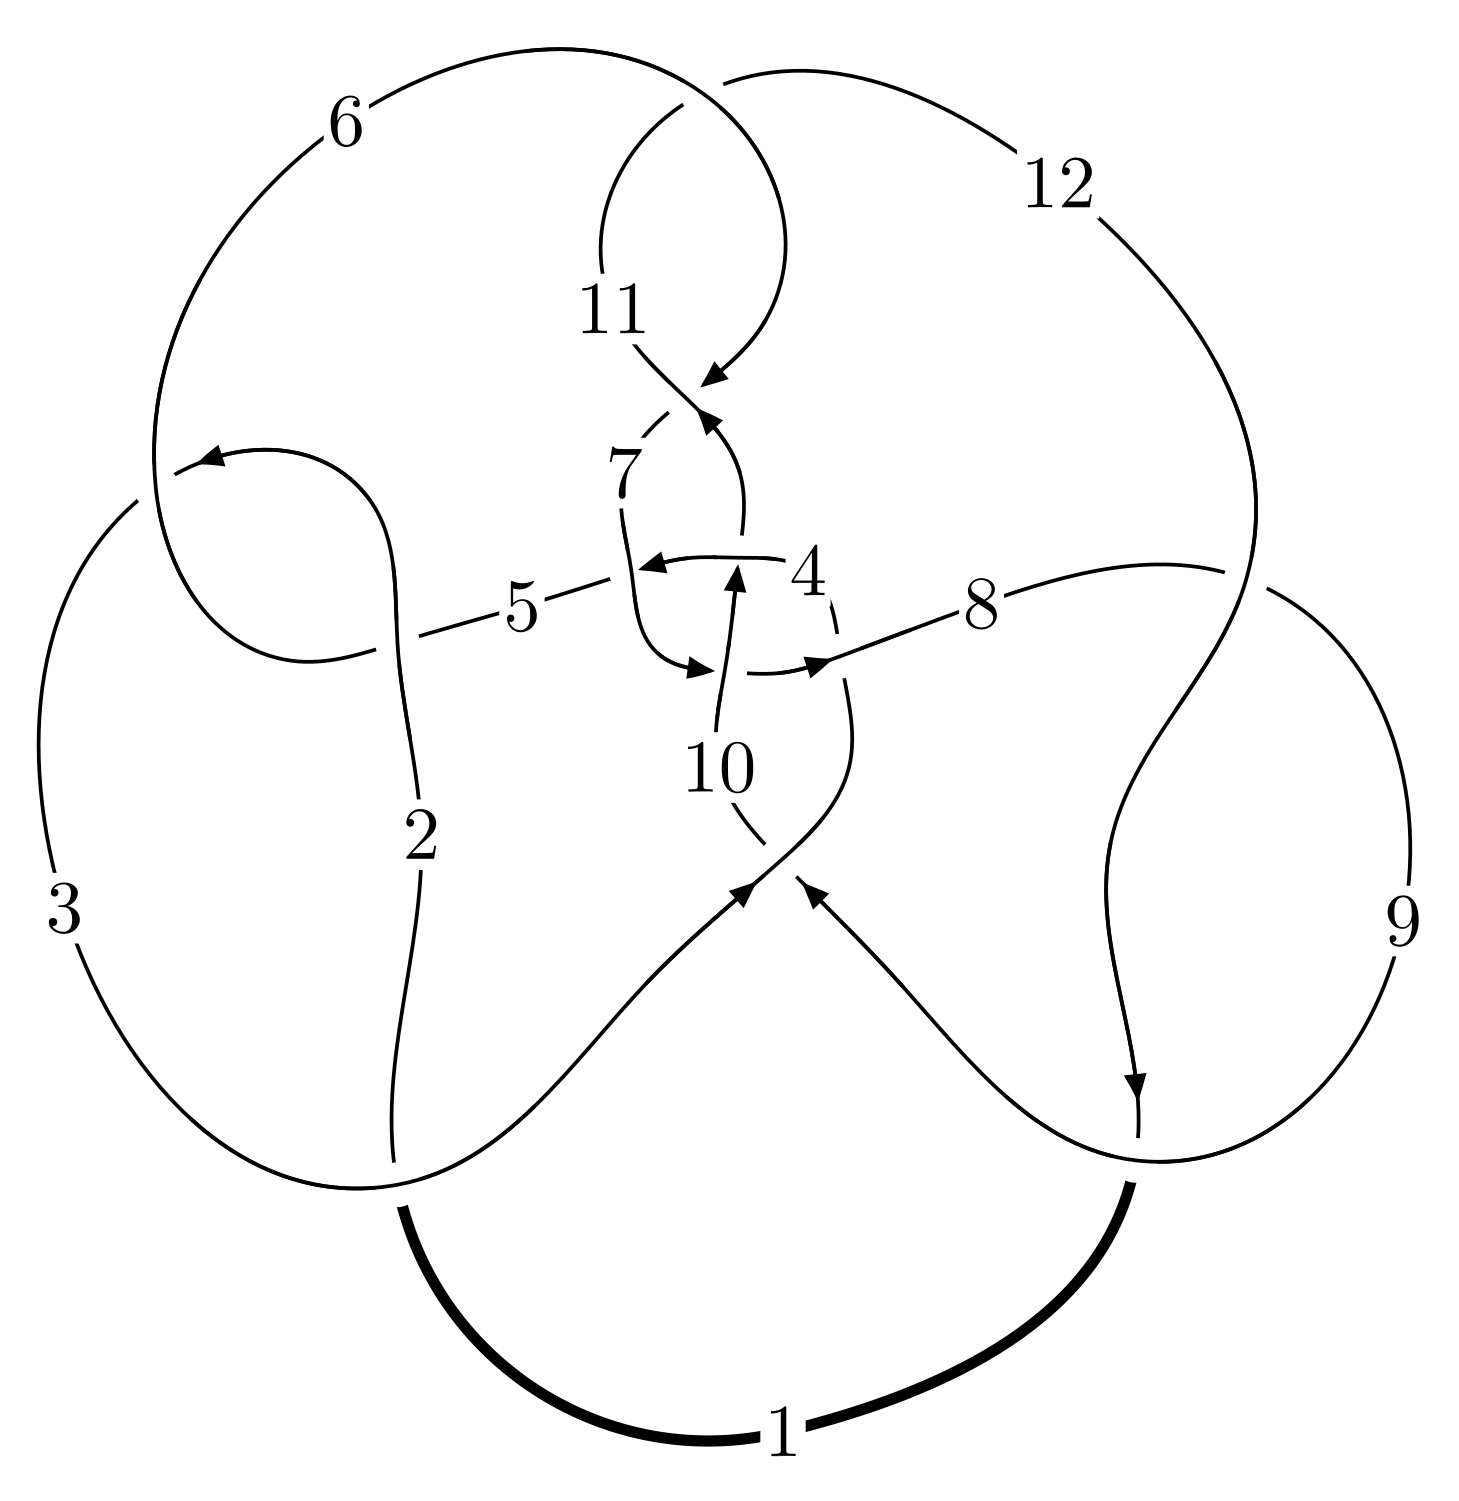
\includegraphics[width=112pt]{../../../GIT/diagram.site/Diagrams/png/2615_12n_0526.png}\\
\ \ \ A knot diagram\footnotemark}&
\allowdisplaybreaks
\textbf{Linearized knot diagam} \\
\cline{2-2}
 &
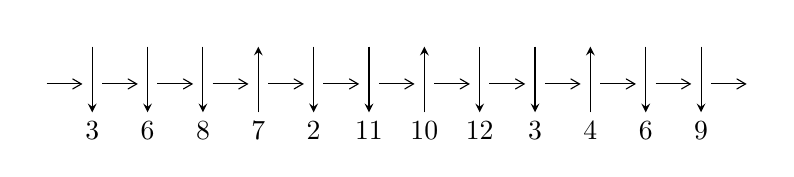
\begin{tikzpicture}[x=20pt, y=17pt]
	% nodes
	\node (C0) at (0, 0) {};
	\node (C1) at (1, 0) {};
	\node (C1U) at (1, +1) {};
	\node (C1D) at (1, -1) {3};

	\node (C2) at (2, 0) {};
	\node (C2U) at (2, +1) {};
	\node (C2D) at (2, -1) {6};

	\node (C3) at (3, 0) {};
	\node (C3U) at (3, +1) {};
	\node (C3D) at (3, -1) {8};

	\node (C4) at (4, 0) {};
	\node (C4U) at (4, +1) {};
	\node (C4D) at (4, -1) {7};

	\node (C5) at (5, 0) {};
	\node (C5U) at (5, +1) {};
	\node (C5D) at (5, -1) {2};

	\node (C6) at (6, 0) {};
	\node (C6U) at (6, +1) {};
	\node (C6D) at (6, -1) {11};

	\node (C7) at (7, 0) {};
	\node (C7U) at (7, +1) {};
	\node (C7D) at (7, -1) {10};

	\node (C8) at (8, 0) {};
	\node (C8U) at (8, +1) {};
	\node (C8D) at (8, -1) {12};

	\node (C9) at (9, 0) {};
	\node (C9U) at (9, +1) {};
	\node (C9D) at (9, -1) {3};

	\node (C10) at (10, 0) {};
	\node (C10U) at (10, +1) {};
	\node (C10D) at (10, -1) {4};

	\node (C11) at (11, 0) {};
	\node (C11U) at (11, +1) {};
	\node (C11D) at (11, -1) {6};

	\node (C12) at (12, 0) {};
	\node (C12U) at (12, +1) {};
	\node (C12D) at (12, -1) {9};
	\node (C13) at (13, 0) {};

	% arrows
	\draw[->,>={angle 60}]
	(C0) edge (C1) (C1) edge (C2) (C2) edge (C3) (C3) edge (C4) (C4) edge (C5) (C5) edge (C6) (C6) edge (C7) (C7) edge (C8) (C8) edge (C9) (C9) edge (C10) (C10) edge (C11) (C11) edge (C12) (C12) edge (C13) ;	\draw[->,>=stealth]
	(C1U) edge (C1D) (C2U) edge (C2D) (C3U) edge (C3D) (C4D) edge (C4U) (C5U) edge (C5D) (C6U) edge (C6D) (C7D) edge (C7U) (C8U) edge (C8D) (C9U) edge (C9D) (C10D) edge (C10U) (C11U) edge (C11D) (C12U) edge (C12D) ;
	\end{tikzpicture} \\
\hhline{~~} \\& 
\textbf{Solving Sequence} \\ \cline{2-2} 
 &
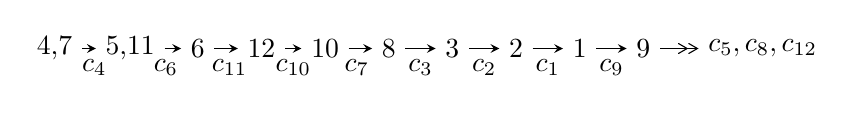
\begin{tikzpicture}[x=23pt, y=7pt]
	% node
	\node (A0) at (-1/8, 0) {4,7};
	\node (A1) at (17/16, 0) {5,11};
	\node (A2) at (17/8, 0) {6};
	\node (A3) at (25/8, 0) {12};
	\node (A4) at (33/8, 0) {10};
	\node (A5) at (41/8, 0) {8};
	\node (A6) at (49/8, 0) {3};
	\node (A7) at (57/8, 0) {2};
	\node (A8) at (65/8, 0) {1};
	\node (A9) at (73/8, 0) {9};
	\node (C1) at (1/2, -1) {$c_{4}$};
	\node (C2) at (13/8, -1) {$c_{6}$};
	\node (C3) at (21/8, -1) {$c_{11}$};
	\node (C4) at (29/8, -1) {$c_{10}$};
	\node (C5) at (37/8, -1) {$c_{7}$};
	\node (C6) at (45/8, -1) {$c_{3}$};
	\node (C7) at (53/8, -1) {$c_{2}$};
	\node (C8) at (61/8, -1) {$c_{1}$};
	\node (C9) at (69/8, -1) {$c_{9}$};
	\node (A10) at (11, 0) {$c_{5},c_{8},c_{12}$};

	% edge
	\draw[->,>=stealth]	
	(A0) edge (A1) (A1) edge (A2) (A2) edge (A3) (A3) edge (A4) (A4) edge (A5) (A5) edge (A6) (A6) edge (A7) (A7) edge (A8) (A8) edge (A9) ;
	\draw[->>,>={angle 60}]	
	(A9) edge (A10);
\end{tikzpicture} \\ 

\end{tabular} \\

\footnotetext{
The image of knot diagram is generated by the software ``\textbf{Draw programme}" developed by Andrew Bartholomew(\url{http://www.layer8.co.uk/maths/draw/index.htm\#Running-draw}), where we modified some parts for our purpose(\url{https://github.com/CATsTAILs/LinksPainter}).
}\phantom \\ \newline 
\centering \textbf{Ideals for irreducible components\footnotemark of $X_{\text{par}}$} 
 
\begin{align*}
I^u_{1}&=\langle 
509724805881808 u^{17}+62725492089096 u^{16}+\cdots+962155230401099 b-2566227709173424,\\
\phantom{I^u_{1}}&\phantom{= \langle  }509724805881808 u^{17}+62725492089096 u^{16}+\cdots+962155230401099 a-1604072478772325,\\
\phantom{I^u_{1}}&\phantom{= \langle  }u^{18}+13 u^{15}+\cdots-3 u+1\rangle \\
I^u_{2}&=\langle 
-2 u^3+u^2+5 b+7 u+4,\;-2 u^3+u^2+5 a+7 u+9,\;u^4- u^3-2 u^2-4 u+1\rangle \\
I^u_{3}&=\langle 
-27 u^5-100 u^4-44 u^3+97 u^2+83 b-149 u-351,\\
\phantom{I^u_{3}}&\phantom{= \langle  }151 u^5+341 u^4+160 u^3+598 u^2+1909 a+1153 u+552,\;u^6+5 u^5+7 u^4+2 u^2+23 u+23\rangle \\
I^u_{4}&=\langle 
2.26609\times10^{20} u^{17}-1.36596\times10^{21} u^{16}+\cdots+1.11949\times10^{23} b-1.57690\times10^{23},\\
\phantom{I^u_{4}}&\phantom{= \langle  }-2.09433\times10^{24} u^{17}+1.13703\times10^{25} u^{16}+\cdots+1.33689\times10^{27} a+3.04454\times10^{27},\\
\phantom{I^u_{4}}&\phantom{= \langle  }u^{18}-6 u^{17}+\cdots-1792 u+448\rangle \\
I^u_{5}&=\langle 
- u^5-2 u^4-6 u^3-3 u^2+4 b-5 u+5,\;- u^5-2 u^4-6 u^3-3 u^2+4 a-5 u+5,\\
\phantom{I^u_{5}}&\phantom{= \langle  }u^6+u^5+4 u^4+u^3+2 u^2-2 u+1\rangle \\
\\
I^v_{1}&=\langle 
a,\;3 v^5-2 v^4+15 v^3-20 v^2+7 b+12 v+3,\;v^6- v^5+5 v^4-9 v^3+5 v^2- v+1\rangle \\
\end{align*}
\raggedright * 6 irreducible components of $\dim_{\mathbb{C}}=0$, with total 58 representations.\\
\footnotetext{All coefficients of polynomials are rational numbers. But the coefficients are sometimes approximated in decimal forms when there is not enough margin.}
\newpage
\renewcommand{\arraystretch}{1}
\centering \section*{I. $I^u_{1}= \langle 5.10\times10^{14} u^{17}+6.27\times10^{13} u^{16}+\cdots+9.62\times10^{14} b-2.57\times10^{15},\;5.10\times10^{14} u^{17}+6.27\times10^{13} u^{16}+\cdots+9.62\times10^{14} a-1.60\times10^{15},\;u^{18}+13 u^{15}+\cdots-3 u+1 \rangle$}
\flushleft \textbf{(i) Arc colorings}\\
\begin{tabular}{m{7pt} m{180pt} m{7pt} m{180pt} }
\flushright $a_{4}=$&$\begin{pmatrix}1\\0\end{pmatrix}$ \\
\flushright $a_{7}=$&$\begin{pmatrix}0\\u\end{pmatrix}$ \\
\flushright $a_{5}=$&$\begin{pmatrix}1\\- u^2\end{pmatrix}$ \\
\flushright $a_{11}=$&$\begin{pmatrix}-0.529774 u^{17}-0.0651927 u^{16}+\cdots-10.5792 u+1.66717\\-0.529774 u^{17}-0.0651927 u^{16}+\cdots-10.5792 u+2.66717\end{pmatrix}$ \\
\flushright $a_{6}=$&$\begin{pmatrix}0.0770104 u^{17}+0.260613 u^{16}+\cdots-4.25101 u+1.18675\\0.0118177 u^{17}+0.255567 u^{16}+\cdots-3.17317 u+1.71652\end{pmatrix}$ \\
\flushright $a_{12}=$&$\begin{pmatrix}-1.25969 u^{17}+0.0649203 u^{16}+\cdots-13.8506 u+2.19363\\-1.00412 u^{17}+0.0243057 u^{16}+\cdots-12.0986 u+3.18181\end{pmatrix}$ \\
\flushright $a_{10}=$&$\begin{pmatrix}-1\\-0.529774 u^{17}-0.0651927 u^{16}+\cdots-10.5792 u+2.66717\end{pmatrix}$ \\
\flushright $a_{8}=$&$\begin{pmatrix}u\\0.0651927 u^{17}+0.00504605 u^{16}+\cdots-0.0778441 u-0.529774\end{pmatrix}$ \\
\flushright $a_{3}=$&$\begin{pmatrix}-0.00504605 u^{17}+0.0633402 u^{16}+\cdots+0.334196 u+1.06519\\-0.260613 u^{17}+0.103955 u^{16}+\cdots-1.41778 u+0.0770104\end{pmatrix}$ \\
\flushright $a_{2}=$&$\begin{pmatrix}0.471649 u^{17}+0.309437 u^{16}+\cdots+1.48208 u+1.26622\\0.0769485 u^{17}+0.231016 u^{16}+\cdots-0.716691 u-0.529509\end{pmatrix}$ \\
\flushright $a_{1}=$&$\begin{pmatrix}0.526910 u^{17}+0.0682034 u^{16}+\cdots+4.16343 u-0.388870\\0.108885 u^{17}+0.0443291 u^{16}+\cdots+0.972123 u-0.838062\end{pmatrix}$ \\
\flushright $a_{9}=$&$\begin{pmatrix}-0.386278 u^{17}+0.00755787 u^{16}+\cdots-9.06550 u+1.82450\\-0.335639 u^{17}-0.0387286 u^{16}+\cdots-9.84582 u+2.34782\end{pmatrix}$\\&\end{tabular}
\flushleft \textbf{(ii) Obstruction class $= -1$}\\~\\
\flushleft \textbf{(iii) Cusp Shapes $= -\frac{10294514371764425}{962155230401099} u^{17}-\frac{6856664502715686}{962155230401099} u^{16}+\cdots-\frac{99549238607210006}{962155230401099} u-\frac{114009180214742949}{962155230401099}$}\\~\\
\newpage\renewcommand{\arraystretch}{1}
\flushleft \textbf{(iv) u-Polynomials at the component}\newline \\
\begin{tabular}{m{50pt}|m{274pt}}
Crossings & \hspace{64pt}u-Polynomials at each crossing \\
\hline $$\begin{aligned}c_{1}\end{aligned}$$&$\begin{aligned}
&u^{18}+20 u^{17}+\cdots+9 u+1
\end{aligned}$\\
\hline $$\begin{aligned}c_{2},c_{5},c_{8}\\c_{12}\end{aligned}$$&$\begin{aligned}
&u^{18}-10 u^{16}+\cdots+u+1
\end{aligned}$\\
\hline $$\begin{aligned}c_{3},c_{6},c_{11}\end{aligned}$$&$\begin{aligned}
&u^{18}+4 u^{16}+\cdots-5 u+1
\end{aligned}$\\
\hline $$\begin{aligned}c_{4},c_{7}\end{aligned}$$&$\begin{aligned}
&u^{18}-13 u^{15}+\cdots+3 u+1
\end{aligned}$\\
\hline $$\begin{aligned}c_{9}\end{aligned}$$&$\begin{aligned}
&u^{18}+4 u^{17}+\cdots+2 u+49
\end{aligned}$\\
\hline $$\begin{aligned}c_{10}\end{aligned}$$&$\begin{aligned}
&u^{18}+11 u^{17}+\cdots+12 u+7
\end{aligned}$\\
\hline
\end{tabular}\\~\\
\newpage\renewcommand{\arraystretch}{1}
\flushleft \textbf{(v) Riley Polynomials at the component}\newline \\
\begin{tabular}{m{50pt}|m{274pt}}
Crossings & \hspace{64pt}Riley Polynomials at each crossing \\
\hline $$\begin{aligned}c_{1}\end{aligned}$$&$\begin{aligned}
&y^{18}-44 y^{17}+\cdots+123 y+1
\end{aligned}$\\
\hline $$\begin{aligned}c_{2},c_{5},c_{8}\\c_{12}\end{aligned}$$&$\begin{aligned}
&y^{18}-20 y^{17}+\cdots-9 y+1
\end{aligned}$\\
\hline $$\begin{aligned}c_{3},c_{6},c_{11}\end{aligned}$$&$\begin{aligned}
&y^{18}+8 y^{17}+\cdots-13 y+1
\end{aligned}$\\
\hline $$\begin{aligned}c_{4},c_{7}\end{aligned}$$&$\begin{aligned}
&y^{18}+10 y^{16}+\cdots+43 y+1
\end{aligned}$\\
\hline $$\begin{aligned}c_{9}\end{aligned}$$&$\begin{aligned}
&y^{18}-38 y^{17}+\cdots+23516 y+2401
\end{aligned}$\\
\hline $$\begin{aligned}c_{10}\end{aligned}$$&$\begin{aligned}
&y^{18}-7 y^{17}+\cdots-578 y+49
\end{aligned}$\\
\hline
\end{tabular}\\~\\
\newpage\flushleft \textbf{(vi) Complex Volumes and Cusp Shapes}
$$\begin{array}{c|c|c}  
\text{Solutions to }I^u_{1}& \I (\text{vol} + \sqrt{-1}CS) & \text{Cusp shape}\\
 \hline 
\begin{aligned}
u &= -0.113980 + 1.055280 I \\
a &= -1.44079 - 0.05034 I \\
b &= -0.440789 - 0.050343 I\end{aligned}
 & \phantom{-}0.52334 + 2.87308 I & -12.86704 - 2.02894 I \\ \hline\begin{aligned}
u &= -0.113980 - 1.055280 I \\
a &= -1.44079 + 0.05034 I \\
b &= -0.440789 + 0.050343 I\end{aligned}
 & \phantom{-}0.52334 - 2.87308 I & -12.86704 + 2.02894 I \\ \hline\begin{aligned}
u &= \phantom{-}0.954988 + 0.936855 I \\
a &= -0.110942 + 0.898533 I \\
b &= \phantom{-}0.889058 + 0.898533 I\end{aligned}
 & -3.78393 + 7.04028 I & -11.7360 - 7.9578 I \\ \hline\begin{aligned}
u &= \phantom{-}0.954988 - 0.936855 I \\
a &= -0.110942 - 0.898533 I \\
b &= \phantom{-}0.889058 - 0.898533 I\end{aligned}
 & -3.78393 - 7.04028 I & -11.7360 + 7.9578 I \\ \hline\begin{aligned}
u &= -0.058366 + 0.626910 I \\
a &= -1.99797 + 0.34561 I \\
b &= -0.997971 + 0.345611 I\end{aligned}
 & \phantom{-}3.21985 - 4.16919 I & -1.22804 + 6.95897 I \\ \hline\begin{aligned}
u &= -0.058366 - 0.626910 I \\
a &= -1.99797 - 0.34561 I \\
b &= -0.997971 - 0.345611 I\end{aligned}
 & \phantom{-}3.21985 + 4.16919 I & -1.22804 - 6.95897 I \\ \hline\begin{aligned}
u &= \phantom{-}0.705132 + 1.217160 I \\
a &= -0.230297 - 1.183980 I \\
b &= \phantom{-}0.769703 - 1.183980 I\end{aligned}
 & -18.2643 + 6.2926 I & -8.79577 - 2.62001 I \\ \hline\begin{aligned}
u &= \phantom{-}0.705132 - 1.217160 I \\
a &= -0.230297 + 1.183980 I \\
b &= \phantom{-}0.769703 + 1.183980 I\end{aligned}
 & -18.2643 - 6.2926 I & -8.79577 + 2.62001 I \\ \hline\begin{aligned}
u &= -0.92137 + 1.10060 I \\
a &= \phantom{-}0.292045 - 0.754405 I \\
b &= \phantom{-}1.29204 - 0.75441 I\end{aligned}
 & \phantom{-}2.25471 - 6.85293 I & \phantom{-}2.33518 + 2.51828 I \\ \hline\begin{aligned}
u &= -0.92137 - 1.10060 I \\
a &= \phantom{-}0.292045 + 0.754405 I \\
b &= \phantom{-}1.29204 + 0.75441 I\end{aligned}
 & \phantom{-}2.25471 + 6.85293 I & \phantom{-}2.33518 - 2.51828 I\\
 \hline 
 \end{array}$$\newpage$$\begin{array}{c|c|c}  
\text{Solutions to }I^u_{1}& \I (\text{vol} + \sqrt{-1}CS) & \text{Cusp shape}\\
 \hline 
\begin{aligned}
u &= \phantom{-}0.069851 + 0.514524 I \\
a &= -0.761951 + 0.761302 I \\
b &= \phantom{-}0.238049 + 0.761302 I\end{aligned}
 & -0.860650 - 0.772825 I & -7.78859 + 5.59560 I \\ \hline\begin{aligned}
u &= \phantom{-}0.069851 - 0.514524 I \\
a &= -0.761951 - 0.761302 I \\
b &= \phantom{-}0.238049 - 0.761302 I\end{aligned}
 & -0.860650 + 0.772825 I & -7.78859 - 5.59560 I \\ \hline\begin{aligned}
u &= \phantom{-}0.071122 + 0.227795 I \\
a &= \phantom{-}0.79662 - 1.30381 I \\
b &= \phantom{-}1.79662 - 1.30381 I\end{aligned}
 & -2.88172 + 0.11696 I & -86.2726 - 33.4077 I \\ \hline\begin{aligned}
u &= \phantom{-}0.071122 - 0.227795 I \\
a &= \phantom{-}0.79662 + 1.30381 I \\
b &= \phantom{-}1.79662 + 1.30381 I\end{aligned}
 & -2.88172 - 0.11696 I & -86.2726 + 33.4077 I \\ \hline\begin{aligned}
u &= -2.05408 + 0.03763 I \\
a &= -0.195363 + 0.174827 I \\
b &= \phantom{-}0.804637 + 0.174827 I\end{aligned}
 & \phantom{-}5.48543 + 0.72645 I & -2.62157 - 10.03199 I \\ \hline\begin{aligned}
u &= -2.05408 - 0.03763 I \\
a &= -0.195363 - 0.174827 I \\
b &= \phantom{-}0.804637 - 0.174827 I\end{aligned}
 & \phantom{-}5.48543 - 0.72645 I & -2.62157 + 10.03199 I \\ \hline\begin{aligned}
u &= \phantom{-}1.34670 + 1.70942 I \\
a &= \phantom{-}0.148649 + 0.885147 I \\
b &= \phantom{-}1.14865 + 0.88515 I\end{aligned}
 & -16.9465 + 13.6621 I & -7.52555 - 5.67041 I \\ \hline\begin{aligned}
u &= \phantom{-}1.34670 - 1.70942 I \\
a &= \phantom{-}0.148649 - 0.885147 I \\
b &= \phantom{-}1.14865 - 0.88515 I\end{aligned}
 & -16.9465 - 13.6621 I & -7.52555 + 5.67041 I\\
 \hline 
 \end{array}$$\newpage\newpage\renewcommand{\arraystretch}{1}
\centering \section*{II. $I^u_{2}= \langle -2 u^3+u^2+5 b+7 u+4,\;-2 u^3+u^2+5 a+7 u+9,\;u^4- u^3-2 u^2-4 u+1 \rangle$}
\flushleft \textbf{(i) Arc colorings}\\
\begin{tabular}{m{7pt} m{180pt} m{7pt} m{180pt} }
\flushright $a_{4}=$&$\begin{pmatrix}1\\0\end{pmatrix}$ \\
\flushright $a_{7}=$&$\begin{pmatrix}0\\u\end{pmatrix}$ \\
\flushright $a_{5}=$&$\begin{pmatrix}1\\- u^2\end{pmatrix}$ \\
\flushright $a_{11}=$&$\begin{pmatrix}\frac{2}{5} u^3-\frac{1}{5} u^2-\frac{7}{5} u-\frac{9}{5}\\\frac{2}{5} u^3-\frac{1}{5} u^2-\frac{7}{5} u-\frac{4}{5}\end{pmatrix}$ \\
\flushright $a_{6}=$&$\begin{pmatrix}1\\\frac{1}{5} u^3-\frac{3}{5} u^2+\frac{4}{5} u+\frac{3}{5}\end{pmatrix}$ \\
\flushright $a_{12}=$&$\begin{pmatrix}\frac{3}{5} u^3-\frac{4}{5} u^2-\frac{8}{5} u-\frac{11}{5}\\\frac{1}{5} u^3-\frac{3}{5} u^2-\frac{1}{5} u-\frac{7}{5}\end{pmatrix}$ \\
\flushright $a_{10}=$&$\begin{pmatrix}-1\\\frac{2}{5} u^3-\frac{1}{5} u^2-\frac{7}{5} u-\frac{4}{5}\end{pmatrix}$ \\
\flushright $a_{8}=$&$\begin{pmatrix}u\\-\frac{1}{5} u^3+\frac{3}{5} u^2+\frac{1}{5} u+\frac{2}{5}\end{pmatrix}$ \\
\flushright $a_{3}=$&$\begin{pmatrix}-\frac{2}{5} u^3+\frac{1}{5} u^2+\frac{2}{5} u+\frac{4}{5}\\- u\end{pmatrix}$ \\
\flushright $a_{2}=$&$\begin{pmatrix}0\\\frac{2}{5} u^3-\frac{1}{5} u^2-\frac{2}{5} u-\frac{4}{5}\end{pmatrix}$ \\
\flushright $a_{1}=$&$\begin{pmatrix}u^3+u^2+u-1\\u^3+u^2+u-1\end{pmatrix}$ \\
\flushright $a_{9}=$&$\begin{pmatrix}\frac{3}{5} u^3+\frac{1}{5} u^2+\frac{2}{5} u-\frac{11}{5}\\\frac{2}{5} u^3+\frac{4}{5} u^2-\frac{2}{5} u-\frac{4}{5}\end{pmatrix}$\\&\end{tabular}
\flushleft \textbf{(ii) Obstruction class $= 1$}\\~\\
\flushleft \textbf{(iii) Cusp Shapes $= \frac{13}{5} u^3-\frac{29}{5} u^2+\frac{7}{5} u-\frac{91}{5}$}\\~\\
\newpage\renewcommand{\arraystretch}{1}
\flushleft \textbf{(iv) u-Polynomials at the component}\newline \\
\begin{tabular}{m{50pt}|m{274pt}}
Crossings & \hspace{64pt}u-Polynomials at each crossing \\
\hline $$\begin{aligned}c_{1}\end{aligned}$$&$\begin{aligned}
&u^4-9 u^3+10 u^2-4 u+1
\end{aligned}$\\
\hline $$\begin{aligned}c_{2},c_{8}\end{aligned}$$&$\begin{aligned}
&u^4+3 u^3-2 u-1
\end{aligned}$\\
\hline $$\begin{aligned}c_{3},c_{6}\end{aligned}$$&$\begin{aligned}
&u^4- u^3-2 u+1
\end{aligned}$\\
\hline $$\begin{aligned}c_{4},c_{7}\end{aligned}$$&$\begin{aligned}
&u^4- u^3-2 u^2-4 u+1
\end{aligned}$\\
\hline $$\begin{aligned}c_{5},c_{12}\end{aligned}$$&$\begin{aligned}
&u^4-3 u^3+2 u-1
\end{aligned}$\\
\hline $$\begin{aligned}c_{9}\end{aligned}$$&$\begin{aligned}
&u^4-5 u^3+7 u^2-7 u+5
\end{aligned}$\\
\hline $$\begin{aligned}c_{10}\end{aligned}$$&$\begin{aligned}
&u^4+2 u^3-3 u-1
\end{aligned}$\\
\hline $$\begin{aligned}c_{11}\end{aligned}$$&$\begin{aligned}
&u^4+u^3+2 u+1
\end{aligned}$\\
\hline
\end{tabular}\\~\\
\newpage\renewcommand{\arraystretch}{1}
\flushleft \textbf{(v) Riley Polynomials at the component}\newline \\
\begin{tabular}{m{50pt}|m{274pt}}
Crossings & \hspace{64pt}Riley Polynomials at each crossing \\
\hline $$\begin{aligned}c_{1}\end{aligned}$$&$\begin{aligned}
&y^4-61 y^3+30 y^2+4 y+1
\end{aligned}$\\
\hline $$\begin{aligned}c_{2},c_{5},c_{8}\\c_{12}\end{aligned}$$&$\begin{aligned}
&y^4-9 y^3+10 y^2-4 y+1
\end{aligned}$\\
\hline $$\begin{aligned}c_{3},c_{6},c_{11}\end{aligned}$$&$\begin{aligned}
&y^4- y^3-2 y^2-4 y+1
\end{aligned}$\\
\hline $$\begin{aligned}c_{4},c_{7}\end{aligned}$$&$\begin{aligned}
&y^4-5 y^3-2 y^2-20 y+1
\end{aligned}$\\
\hline $$\begin{aligned}c_{9}\end{aligned}$$&$\begin{aligned}
&y^4-11 y^3-11 y^2+21 y+25
\end{aligned}$\\
\hline $$\begin{aligned}c_{10}\end{aligned}$$&$\begin{aligned}
&y^4-4 y^3+10 y^2-9 y+1
\end{aligned}$\\
\hline
\end{tabular}\\~\\
\newpage\flushleft \textbf{(vi) Complex Volumes and Cusp Shapes}
$$\begin{array}{c|c|c}  
\text{Solutions to }I^u_{2}& \I (\text{vol} + \sqrt{-1}CS) & \text{Cusp shape}\\
 \hline 
\begin{aligned}
u &= -0.826702 + 1.077850 I \\
a &= \phantom{-}0.379567 - 0.769480 I \\
b &= \phantom{-}1.37957 - 0.76948 I\end{aligned}
 & \phantom{-}1.92551 - 7.16341 I & -10.5607 + 14.3354 I \\ \hline\begin{aligned}
u &= -0.826702 - 1.077850 I \\
a &= \phantom{-}0.379567 + 0.769480 I \\
b &= \phantom{-}1.37957 + 0.76948 I\end{aligned}
 & \phantom{-}1.92551 + 7.16341 I & -10.5607 - 14.3354 I \\ \hline\begin{aligned}
u &= \phantom{-}0.222985\phantom{ +0.000000I} \\
a &= -2.11769\phantom{ +0.000000I} \\
b &= -1.11769\phantom{ +0.000000I}\end{aligned}
 & -2.81853\phantom{ +0.000000I} & -18.1470\phantom{ +0.000000I} \\ \hline\begin{aligned}
u &= \phantom{-}2.43042\phantom{ +0.000000I} \\
a &= -0.641445\phantom{ +0.000000I} \\
b &= \phantom{-}0.358555\phantom{ +0.000000I}\end{aligned}
 & -14.1920\phantom{ +0.000000I} & -11.7310\phantom{ +0.000000I}\\
 \hline 
 \end{array}$$\newpage\newpage\renewcommand{\arraystretch}{1}
\centering \section*{III. $I^u_{3}= \langle -27 u^5-100 u^4+\cdots+83 b-351,\;151 u^5+341 u^4+\cdots+1909 a+552,\;u^6+5 u^5+7 u^4+2 u^2+23 u+23 \rangle$}
\flushleft \textbf{(i) Arc colorings}\\
\begin{tabular}{m{7pt} m{180pt} m{7pt} m{180pt} }
\flushright $a_{4}=$&$\begin{pmatrix}1\\0\end{pmatrix}$ \\
\flushright $a_{7}=$&$\begin{pmatrix}0\\u\end{pmatrix}$ \\
\flushright $a_{5}=$&$\begin{pmatrix}1\\- u^2\end{pmatrix}$ \\
\flushright $a_{11}=$&$\begin{pmatrix}-0.0790990 u^{5}-0.178628 u^{4}+\cdots-0.603981 u-0.289157\\0.325301 u^{5}+1.20482 u^{4}+\cdots+1.79518 u+4.22892\end{pmatrix}$ \\
\flushright $a_{6}=$&$\begin{pmatrix}-0.129387 u^{5}-0.418020 u^{4}+\cdots-1.45155 u-1.63855\\0.0843373 u^{5}+0.349398 u^{4}+\cdots+0.650602 u+1.09639\end{pmatrix}$ \\
\flushright $a_{12}=$&$\begin{pmatrix}-0.0314301 u^{5}-0.0246202 u^{4}+\cdots-1.27973 u-0.843373\\-0.216867 u^{5}-0.469880 u^{4}+\cdots-1.53012 u-1.81928\end{pmatrix}$ \\
\flushright $a_{10}=$&$\begin{pmatrix}-0.404400 u^{5}-1.38345 u^{4}+\cdots-2.39916 u-4.51807\\0.325301 u^{5}+1.20482 u^{4}+\cdots+1.79518 u+4.22892\end{pmatrix}$ \\
\flushright $a_{8}=$&$\begin{pmatrix}-0.430592 u^{5}-1.23730 u^{4}+\cdots-1.63227 u-3.55422\\0.216867 u^{5}+0.469880 u^{4}+\cdots+1.53012 u+0.819277\end{pmatrix}$ \\
\flushright $a_{3}=$&$\begin{pmatrix}0.220534 u^{5}+0.789419 u^{4}+\cdots+1.86276 u+3.08434\\0.204819 u^{5}+0.277108 u^{4}+\cdots+1.72289 u-0.337349\end{pmatrix}$ \\
\flushright $a_{2}=$&$\begin{pmatrix}0.315872 u^{5}+1.09743 u^{4}+\cdots+1.51126 u+3.97590\\-0.397590 u^{5}-1.36145 u^{4}+\cdots-1.63855 u-7.16867\end{pmatrix}$ \\
\flushright $a_{1}=$&$\begin{pmatrix}0.358303 u^{5}+1.08067 u^{4}+\cdots+0.788895 u+3.61446\\-0.0963855 u^{5}-0.542169 u^{4}+\cdots-0.457831 u-5.25301\end{pmatrix}$ \\
\flushright $a_{9}=$&$\begin{pmatrix}-0.474070 u^{5}-1.45469 u^{4}+\cdots-1.71922 u-3.55422\\0.132530 u^{5}+0.120482 u^{4}+\cdots+0.879518 u-1.27711\end{pmatrix}$\\&\end{tabular}
\flushleft \textbf{(ii) Obstruction class $= 1$}\\~\\
\flushleft \textbf{(iii) Cusp Shapes $= \frac{109}{83} u^5+\frac{416}{83} u^4+\frac{193}{83} u^3-\frac{450}{83} u^2+\frac{580}{83} u+\frac{1168}{83}$}\\~\\
\newpage\renewcommand{\arraystretch}{1}
\flushleft \textbf{(iv) u-Polynomials at the component}\newline \\
\begin{tabular}{m{50pt}|m{274pt}}
Crossings & \hspace{64pt}u-Polynomials at each crossing \\
\hline $$\begin{aligned}c_{1}\end{aligned}$$&$\begin{aligned}
&u^6- u^5-8 u^4+2 u^3+20 u^2+8 u+1
\end{aligned}$\\
\hline $$\begin{aligned}c_{2},c_{8}\end{aligned}$$&$\begin{aligned}
&u^6+3 u^5+4 u^4+6 u^3+6 u^2+2 u+1
\end{aligned}$\\
\hline $$\begin{aligned}c_{3},c_{6}\end{aligned}$$&$\begin{aligned}
&u^6+3 u^5+4 u^4+3 u^3+3 u^2+2 u+1
\end{aligned}$\\
\hline $$\begin{aligned}c_{4},c_{7}\end{aligned}$$&$\begin{aligned}
&u^6+5 u^5+7 u^4+2 u^2+23 u+23
\end{aligned}$\\
\hline $$\begin{aligned}c_{5},c_{12}\end{aligned}$$&$\begin{aligned}
&u^6-3 u^5+4 u^4-6 u^3+6 u^2-2 u+1
\end{aligned}$\\
\hline $$\begin{aligned}c_{9}\end{aligned}$$&$\begin{aligned}
&u^6+2 u^5+4 u^4+6 u^3+4 u^2+5 u+5
\end{aligned}$\\
\hline $$\begin{aligned}c_{10}\end{aligned}$$&$\begin{aligned}
&(u^3- u^2+1)^2
\end{aligned}$\\
\hline $$\begin{aligned}c_{11}\end{aligned}$$&$\begin{aligned}
&u^6-3 u^5+4 u^4-3 u^3+3 u^2-2 u+1
\end{aligned}$\\
\hline
\end{tabular}\\~\\
\newpage\renewcommand{\arraystretch}{1}
\flushleft \textbf{(v) Riley Polynomials at the component}\newline \\
\begin{tabular}{m{50pt}|m{274pt}}
Crossings & \hspace{64pt}Riley Polynomials at each crossing \\
\hline $$\begin{aligned}c_{1}\end{aligned}$$&$\begin{aligned}
&y^6-17 y^5+108 y^4-306 y^3+352 y^2-24 y+1
\end{aligned}$\\
\hline $$\begin{aligned}c_{2},c_{5},c_{8}\\c_{12}\end{aligned}$$&$\begin{aligned}
&y^6- y^5-8 y^4+2 y^3+20 y^2+8 y+1
\end{aligned}$\\
\hline $$\begin{aligned}c_{3},c_{6},c_{11}\end{aligned}$$&$\begin{aligned}
&y^6- y^5+4 y^4+5 y^3+5 y^2+2 y+1
\end{aligned}$\\
\hline $$\begin{aligned}c_{4},c_{7}\end{aligned}$$&$\begin{aligned}
&y^6-11 y^5+53 y^4-156 y^3+326 y^2-437 y+529
\end{aligned}$\\
\hline $$\begin{aligned}c_{9}\end{aligned}$$&$\begin{aligned}
&y^6+4 y^5-14 y^3-4 y^2+15 y+25
\end{aligned}$\\
\hline $$\begin{aligned}c_{10}\end{aligned}$$&$\begin{aligned}
&(y^3- y^2+2 y-1)^2
\end{aligned}$\\
\hline
\end{tabular}\\~\\
\newpage\flushleft \textbf{(vi) Complex Volumes and Cusp Shapes}
$$\begin{array}{c|c|c}  
\text{Solutions to }I^u_{3}& \I (\text{vol} + \sqrt{-1}CS) & \text{Cusp shape}\\
 \hline 
\begin{aligned}
u &= \phantom{-}0.988837 + 0.990669 I \\
a &= \phantom{-}0.262508 - 1.069710 I \\
b &= -0.877439 - 0.744862 I\end{aligned}
 & -2.75839 + 5.65624 I & -7.72484 - 4.28659 I \\ \hline\begin{aligned}
u &= \phantom{-}0.988837 - 0.990669 I \\
a &= \phantom{-}0.262508 + 1.069710 I \\
b &= -0.877439 + 0.744862 I\end{aligned}
 & -2.75839 - 5.65624 I & -7.72484 + 4.28659 I \\ \hline\begin{aligned}
u &= -1.44904 + 0.80809 I \\
a &= -0.066092 + 0.513653 I \\
b &= -0.877439 + 0.744862 I\end{aligned}
 & -2.75839 - 5.65624 I & -7.72484 + 4.28659 I \\ \hline\begin{aligned}
u &= -1.44904 - 0.80809 I \\
a &= -0.066092 - 0.513653 I \\
b &= -0.877439 - 0.744862 I\end{aligned}
 & -2.75839 + 5.65624 I & -7.72484 - 4.28659 I \\ \hline\begin{aligned}
u &= -2.03980 + 0.32227 I \\
a &= -0.196416 - 0.308287 I \\
b &= \phantom{-}0.754878\phantom{ +0.000000I}\end{aligned}
 & \phantom{-}5.51678\phantom{ +0.000000I} & -1.55033 + 0. I\phantom{ +0.000000I} \\ \hline\begin{aligned}
u &= -2.03980 - 0.32227 I \\
a &= -0.196416 + 0.308287 I \\
b &= \phantom{-}0.754878\phantom{ +0.000000I}\end{aligned}
 & \phantom{-}5.51678\phantom{ +0.000000I} & -1.55033 + 0. I\phantom{ +0.000000I}\\
 \hline 
 \end{array}$$\newpage\newpage\renewcommand{\arraystretch}{1}
\centering \section*{IV. $I^u_{4}= \langle 2.27\times10^{20} u^{17}-1.37\times10^{21} u^{16}+\cdots+1.12\times10^{23} b-1.58\times10^{23},\;-2.09\times10^{24} u^{17}+1.14\times10^{25} u^{16}+\cdots+1.34\times10^{27} a+3.04\times10^{27},\;u^{18}-6 u^{17}+\cdots-1792 u+448 \rangle$}
\flushleft \textbf{(i) Arc colorings}\\
\begin{tabular}{m{7pt} m{180pt} m{7pt} m{180pt} }
\flushright $a_{4}=$&$\begin{pmatrix}1\\0\end{pmatrix}$ \\
\flushright $a_{7}=$&$\begin{pmatrix}0\\u\end{pmatrix}$ \\
\flushright $a_{5}=$&$\begin{pmatrix}1\\- u^2\end{pmatrix}$ \\
\flushright $a_{11}=$&$\begin{pmatrix}0.00156657 u^{17}-0.00850503 u^{16}+\cdots+2.44857 u-2.27733\\-0.00202422 u^{17}+0.0122017 u^{16}+\cdots-3.29503 u+1.40859\end{pmatrix}$ \\
\flushright $a_{6}=$&$\begin{pmatrix}-0.000637368 u^{17}+0.00640601 u^{16}+\cdots-5.05787 u+2.59216\\0.000789287 u^{17}-0.00442185 u^{16}+\cdots+1.05475 u-0.409876\end{pmatrix}$ \\
\flushright $a_{12}=$&$\begin{pmatrix}0.00561057 u^{17}-0.0351617 u^{16}+\cdots+10.1022 u-4.69092\\-0.00341981 u^{17}+0.0194053 u^{16}+\cdots-3.19877 u+1.32313\end{pmatrix}$ \\
\flushright $a_{10}=$&$\begin{pmatrix}0.00359079 u^{17}-0.0207067 u^{16}+\cdots+5.74360 u-3.68591\\-0.00202422 u^{17}+0.0122017 u^{16}+\cdots-3.29503 u+1.40859\end{pmatrix}$ \\
\flushright $a_{8}=$&$\begin{pmatrix}-0.00281027 u^{17}+0.0171228 u^{16}+\cdots-3.36307 u+2.95981\\0.00138362 u^{17}-0.00629498 u^{16}+\cdots-0.749549 u+0.0422281\end{pmatrix}$ \\
\flushright $a_{3}=$&$\begin{pmatrix}-0.00357012 u^{17}+0.0247277 u^{16}+\cdots-10.0442 u+4.09627\\0.00217249 u^{17}-0.0135804 u^{16}+\cdots+3.24713 u-0.842978\end{pmatrix}$ \\
\flushright $a_{2}=$&$\begin{pmatrix}-0.00271628 u^{17}+0.0142865 u^{16}+\cdots-2.16712 u+2.24397\\-0.0000227747 u^{17}-0.000799890 u^{16}+\cdots+1.37886 u-0.473454\end{pmatrix}$ \\
\flushright $a_{1}=$&$\begin{pmatrix}0.00709297 u^{17}-0.0701956 u^{16}+\cdots+37.8937 u-7.60167\\-0.00852875 u^{17}+0.0481617 u^{16}+\cdots-1.21841 u-0.548662\end{pmatrix}$ \\
\flushright $a_{9}=$&$\begin{pmatrix}-0.00489348 u^{17}+0.0417001 u^{16}+\cdots-18.1725 u+3.79994\\0.00382063 u^{17}-0.0210140 u^{16}+\cdots-0.151573 u+0.959736\end{pmatrix}$\\&\end{tabular}
\flushleft \textbf{(ii) Obstruction class $= -1$}\\~\\
\flushleft \textbf{(iii) Cusp Shapes $= -\frac{34240253580128948442025}{5968267629674793473663576} u^{17}+\frac{858353517483104921035359}{23873070518699173894654304} u^{16}+\cdots-\frac{31952090119299828142911655}{2984133814837396736831788} u-\frac{315919293533464455836207}{746033453709349184207947}$}\\~\\
\newpage\renewcommand{\arraystretch}{1}
\flushleft \textbf{(iv) u-Polynomials at the component}\newline \\
\begin{tabular}{m{50pt}|m{274pt}}
Crossings & \hspace{64pt}u-Polynomials at each crossing \\
\hline $$\begin{aligned}c_{1}\end{aligned}$$&$\begin{aligned}
&u^{18}+45 u^{17}+\cdots+2548098 u+35721
\end{aligned}$\\
\hline $$\begin{aligned}c_{2},c_{5},c_{8}\\c_{12}\end{aligned}$$&$\begin{aligned}
&u^{18}+u^{17}+\cdots-2016 u+189
\end{aligned}$\\
\hline $$\begin{aligned}c_{3},c_{6},c_{11}\end{aligned}$$&$\begin{aligned}
&u^{18}+2 u^{17}+\cdots-140 u+43
\end{aligned}$\\
\hline $$\begin{aligned}c_{4},c_{7}\end{aligned}$$&$\begin{aligned}
&u^{18}+6 u^{17}+\cdots+1792 u+448
\end{aligned}$\\
\hline $$\begin{aligned}c_{9}\end{aligned}$$&$\begin{aligned}
&u^{18}+4 u^{17}+\cdots-4364 u-2008
\end{aligned}$\\
\hline $$\begin{aligned}c_{10}\end{aligned}$$&$\begin{aligned}
&(u^3- u^2+1)^6
\end{aligned}$\\
\hline
\end{tabular}\\~\\
\newpage\renewcommand{\arraystretch}{1}
\flushleft \textbf{(v) Riley Polynomials at the component}\newline \\
\begin{tabular}{m{50pt}|m{274pt}}
Crossings & \hspace{64pt}Riley Polynomials at each crossing \\
\hline $$\begin{aligned}c_{1}\end{aligned}$$&$\begin{aligned}
&y^{18}-193 y^{17}+\cdots-6886217865618 y+1275989841
\end{aligned}$\\
\hline $$\begin{aligned}c_{2},c_{5},c_{8}\\c_{12}\end{aligned}$$&$\begin{aligned}
&y^{18}-45 y^{17}+\cdots-2548098 y+35721
\end{aligned}$\\
\hline $$\begin{aligned}c_{3},c_{6},c_{11}\end{aligned}$$&$\begin{aligned}
&y^{18}-12 y^{17}+\cdots-25190 y+1849
\end{aligned}$\\
\hline $$\begin{aligned}c_{4},c_{7}\end{aligned}$$&$\begin{aligned}
&y^{18}+12 y^{17}+\cdots-1103872 y+200704
\end{aligned}$\\
\hline $$\begin{aligned}c_{9}\end{aligned}$$&$\begin{aligned}
&y^{18}-48 y^{17}+\cdots-29702960 y+4032064
\end{aligned}$\\
\hline $$\begin{aligned}c_{10}\end{aligned}$$&$\begin{aligned}
&(y^3- y^2+2 y-1)^6
\end{aligned}$\\
\hline
\end{tabular}\\~\\
\newpage\flushleft \textbf{(vi) Complex Volumes and Cusp Shapes}
$$\begin{array}{c|c|c}  
\text{Solutions to }I^u_{4}& \I (\text{vol} + \sqrt{-1}CS) & \text{Cusp shape}\\
 \hline 
\begin{aligned}
u &= \phantom{-}0.932952\phantom{ +0.000000I} \\
a &= \phantom{-}0.372040\phantom{ +0.000000I} \\
b &= \phantom{-}0.754878\phantom{ +0.000000I}\end{aligned}
 & -1.94142\phantom{ +0.000000I} & -2.78240\phantom{ +0.000000I} \\ \hline\begin{aligned}
u &= -0.932140 + 0.590672 I \\
a &= \phantom{-}0.327877 - 0.904251 I \\
b &= \phantom{-}0.754878\phantom{ +0.000000I}\end{aligned}
 & \phantom{-}3.69835\phantom{ +0.000000I} & \phantom{-}                -6
0.266490 + 0. 10   I\phantom{ +0.000000I} \\ \hline\begin{aligned}
u &= -0.932140 - 0.590672 I \\
a &= \phantom{-}0.327877 + 0.904251 I \\
b &= \phantom{-}0.754878\phantom{ +0.000000I}\end{aligned}
 & \phantom{-}3.69835\phantom{ +0.000000I} & \phantom{-}                -6
0.266490 + 0. 10   I\phantom{ +0.000000I} \\ \hline\begin{aligned}
u &= \phantom{-}0.416621 + 0.787171 I \\
a &= \phantom{-}0.712256 - 0.776733 I \\
b &= -0.877439 - 0.744862 I\end{aligned}
 & -0.43923 + 2.82812 I & -6.26278 - 2.97945 I \\ \hline\begin{aligned}
u &= \phantom{-}0.416621 - 0.787171 I \\
a &= \phantom{-}0.712256 + 0.776733 I \\
b &= -0.877439 + 0.744862 I\end{aligned}
 & -0.43923 - 2.82812 I & -6.26278 + 2.97945 I \\ \hline\begin{aligned}
u &= \phantom{-}0.161200 + 1.140610 I \\
a &= \phantom{-}1.11639 + 1.55047 I \\
b &= -0.877439 + 0.744862 I\end{aligned}
 & -17.3586 - 2.8281 I & -7.95480 + 2.97945 I \\ \hline\begin{aligned}
u &= \phantom{-}0.161200 - 1.140610 I \\
a &= \phantom{-}1.11639 - 1.55047 I \\
b &= -0.877439 - 0.744862 I\end{aligned}
 & -17.3586 + 2.8281 I & -7.95480 - 2.97945 I \\ \hline\begin{aligned}
u &= -0.68739 + 1.23808 I \\
a &= -0.248640 + 0.732255 I \\
b &= -0.877439 + 0.744862 I\end{aligned}
 & -0.43923 - 2.82812 I & -6.26278 + 2.97945 I \\ \hline\begin{aligned}
u &= -0.68739 - 1.23808 I \\
a &= -0.248640 - 0.732255 I \\
b &= -0.877439 - 0.744862 I\end{aligned}
 & -0.43923 + 2.82812 I & -6.26278 - 2.97945 I \\ \hline\begin{aligned}
u &= \phantom{-}0.357169\phantom{ +0.000000I} \\
a &= -1.85720\phantom{ +0.000000I} \\
b &= \phantom{-}0.754878\phantom{ +0.000000I}\end{aligned}
 & -1.94142\phantom{ +0.000000I} & -2.78240\phantom{ +0.000000I}\\
 \hline 
 \end{array}$$\newpage$$\begin{array}{c|c|c}  
\text{Solutions to }I^u_{4}& \I (\text{vol} + \sqrt{-1}CS) & \text{Cusp shape}\\
 \hline 
\begin{aligned}
u &= \phantom{-}1.74158\phantom{ +0.000000I} \\
a &= -1.24447\phantom{ +0.000000I} \\
b &= \phantom{-}0.754878\phantom{ +0.000000I}\end{aligned}
 & -13.2210\phantom{ +0.000000I} & -1.42550\phantom{ +0.000000I} \\ \hline\begin{aligned}
u &= -0.45245 + 1.70936 I \\
a &= \phantom{-}0.320272 + 0.802147 I \\
b &= -0.877439 + 0.744862 I\end{aligned}
 & -6.07901 - 2.82812 I & -9.31169 + 2.97945 I \\ \hline\begin{aligned}
u &= -0.45245 - 1.70936 I \\
a &= \phantom{-}0.320272 - 0.802147 I \\
b &= -0.877439 - 0.744862 I\end{aligned}
 & -6.07901 + 2.82812 I & -9.31169 - 2.97945 I \\ \hline\begin{aligned}
u &= \phantom{-}0.63983 + 2.02141 I \\
a &= -0.044419 - 0.705019 I \\
b &= -0.877439 - 0.744862 I\end{aligned}
 & -6.07901 + 2.82812 I & -9.31169 - 2.97945 I \\ \hline\begin{aligned}
u &= \phantom{-}0.63983 - 2.02141 I \\
a &= -0.044419 + 0.705019 I \\
b &= -0.877439 + 0.744862 I\end{aligned}
 & -6.07901 - 2.82812 I & -9.31169 + 2.97945 I \\ \hline\begin{aligned}
u &= \phantom{-}0.59747 + 2.40404 I \\
a &= -0.446280 - 0.570652 I \\
b &= -0.877439 - 0.744862 I\end{aligned}
 & -17.3586 + 2.8281 I & -7.95480 - 2.97945 I \\ \hline\begin{aligned}
u &= \phantom{-}0.59747 - 2.40404 I \\
a &= -0.446280 + 0.570652 I \\
b &= -0.877439 + 0.744862 I\end{aligned}
 & -17.3586 - 2.8281 I & -7.95480 + 2.97945 I \\ \hline\begin{aligned}
u &= \phantom{-}3.48202\phantom{ +0.000000I} \\
a &= \phantom{-}0.254715\phantom{ +0.000000I} \\
b &= \phantom{-}0.754878\phantom{ +0.000000I}\end{aligned}
 & -13.2210\phantom{ +0.000000I} & -1.42550\phantom{ +0.000000I}\\
 \hline 
 \end{array}$$\newpage\newpage\renewcommand{\arraystretch}{1}
\centering \section*{V. $I^u_{5}= \langle - u^5-2 u^4-6 u^3-3 u^2+4 b-5 u+5,\;- u^5-2 u^4-6 u^3-3 u^2+4 a-5 u+5,\;u^6+u^5+4 u^4+u^3+2 u^2-2 u+1 \rangle$}
\flushleft \textbf{(i) Arc colorings}\\
\begin{tabular}{m{7pt} m{180pt} m{7pt} m{180pt} }
\flushright $a_{4}=$&$\begin{pmatrix}1\\0\end{pmatrix}$ \\
\flushright $a_{7}=$&$\begin{pmatrix}0\\u\end{pmatrix}$ \\
\flushright $a_{5}=$&$\begin{pmatrix}1\\- u^2\end{pmatrix}$ \\
\flushright $a_{11}=$&$\begin{pmatrix}\frac{1}{4} u^5+\frac{1}{2} u^4+\cdots+\frac{5}{4} u-\frac{5}{4}\\\frac{1}{4} u^5+\frac{1}{2} u^4+\cdots+\frac{5}{4} u-\frac{5}{4}\end{pmatrix}$ \\
\flushright $a_{6}=$&$\begin{pmatrix}-\frac{1}{2} u^4-\frac{1}{2} u^3-\frac{3}{2} u^2+\frac{1}{2}\\-\frac{1}{2} u^4-\frac{1}{2} u^3-\frac{3}{2} u^2+u+\frac{1}{2}\end{pmatrix}$ \\
\flushright $a_{12}=$&$\begin{pmatrix}\frac{3}{4} u^5+u^4+\cdots+\frac{3}{4} u-\frac{5}{4}\\u^5+\frac{1}{2} u^4+\cdots+u-\frac{3}{2}\end{pmatrix}$ \\
\flushright $a_{10}=$&$\begin{pmatrix}0\\\frac{1}{4} u^5+\frac{1}{2} u^4+\cdots+\frac{5}{4} u-\frac{5}{4}\end{pmatrix}$ \\
\flushright $a_{8}=$&$\begin{pmatrix}0\\u\end{pmatrix}$ \\
\flushright $a_{3}=$&$\begin{pmatrix}1\\- u^2\end{pmatrix}$ \\
\flushright $a_{2}=$&$\begin{pmatrix}\frac{1}{2} u^4+\frac{1}{2} u^3+\frac{3}{2} u^2+\frac{1}{2}\\\frac{1}{2} u^4+\frac{1}{2} u^3+\frac{1}{2} u^2- u-\frac{1}{2}\end{pmatrix}$ \\
\flushright $a_{1}=$&$\begin{pmatrix}\frac{1}{2} u^4+\frac{1}{2} u^3+\frac{3}{2} u^2-\frac{1}{2}\\\frac{1}{2} u^4+\frac{1}{2} u^3+\frac{3}{2} u^2- u-\frac{1}{2}\end{pmatrix}$ \\
\flushright $a_{9}=$&$\begin{pmatrix}\frac{1}{4} u^5+\frac{1}{2} u^4+\cdots+\frac{5}{4} u-\frac{5}{4}\\u^4+u^3+2 u^2+u-1\end{pmatrix}$\\&\end{tabular}
\flushleft \textbf{(ii) Obstruction class $= 1$}\\~\\
\flushleft \textbf{(iii) Cusp Shapes $= \frac{1}{4} u^5+u^4+3 u^3+\frac{5}{4} u^2+\frac{13}{4} u-\frac{35}{4}$}\\~\\
\newpage\renewcommand{\arraystretch}{1}
\flushleft \textbf{(iv) u-Polynomials at the component}\newline \\
\begin{tabular}{m{50pt}|m{274pt}}
Crossings & \hspace{64pt}u-Polynomials at each crossing \\
\hline $$\begin{aligned}c_{1},c_{2}\end{aligned}$$&$\begin{aligned}
&(u-1)^6
\end{aligned}$\\
\hline $$\begin{aligned}c_{3},c_{4}\end{aligned}$$&$\begin{aligned}
&u^6+u^5+4 u^4+u^3+2 u^2-2 u+1
\end{aligned}$\\
\hline $$\begin{aligned}c_{5}\end{aligned}$$&$\begin{aligned}
&(u+1)^6
\end{aligned}$\\
\hline $$\begin{aligned}c_{6}\end{aligned}$$&$\begin{aligned}
&(u^3- u^2+2 u-1)^2
\end{aligned}$\\
\hline $$\begin{aligned}c_{7}\end{aligned}$$&$\begin{aligned}
&u^6
\end{aligned}$\\
\hline $$\begin{aligned}c_{8}\end{aligned}$$&$\begin{aligned}
&(u^3+u^2-1)^2
\end{aligned}$\\
\hline $$\begin{aligned}c_{9},c_{10},c_{12}\end{aligned}$$&$\begin{aligned}
&(u^3- u^2+1)^2
\end{aligned}$\\
\hline $$\begin{aligned}c_{11}\end{aligned}$$&$\begin{aligned}
&(u^3+u^2+2 u+1)^2
\end{aligned}$\\
\hline
\end{tabular}\\~\\
\newpage\renewcommand{\arraystretch}{1}
\flushleft \textbf{(v) Riley Polynomials at the component}\newline \\
\begin{tabular}{m{50pt}|m{274pt}}
Crossings & \hspace{64pt}Riley Polynomials at each crossing \\
\hline $$\begin{aligned}c_{1},c_{2},c_{5}\end{aligned}$$&$\begin{aligned}
&(y-1)^6
\end{aligned}$\\
\hline $$\begin{aligned}c_{3},c_{4}\end{aligned}$$&$\begin{aligned}
&y^6+7 y^5+18 y^4+21 y^3+16 y^2+1
\end{aligned}$\\
\hline $$\begin{aligned}c_{6},c_{11}\end{aligned}$$&$\begin{aligned}
&(y^3+3 y^2+2 y-1)^2
\end{aligned}$\\
\hline $$\begin{aligned}c_{7}\end{aligned}$$&$\begin{aligned}
&y^6
\end{aligned}$\\
\hline $$\begin{aligned}c_{8},c_{9},c_{10}\\c_{12}\end{aligned}$$&$\begin{aligned}
&(y^3- y^2+2 y-1)^2
\end{aligned}$\\
\hline
\end{tabular}\\~\\
\newpage\flushleft \textbf{(vi) Complex Volumes and Cusp Shapes}
$$\begin{array}{c|c|c}  
\text{Solutions to }I^u_{5}& \I (\text{vol} + \sqrt{-1}CS) & \text{Cusp shape}\\
 \hline 
\begin{aligned}
u &= -0.592519 + 0.986732 I \\
a &= -0.877439 + 0.744862 I \\
b &= -0.877439 + 0.744862 I\end{aligned}
 & \phantom{-}1.37919 - 2.82812 I & -8.07960 + 2.97945 I \\ \hline\begin{aligned}
u &= -0.592519 - 0.986732 I \\
a &= -0.877439 - 0.744862 I \\
b &= -0.877439 - 0.744862 I\end{aligned}
 & \phantom{-}1.37919 + 2.82812 I & -8.07960 - 2.97945 I \\ \hline\begin{aligned}
u &= \phantom{-}0.377439 + 0.320410 I \\
a &= -0.877439 + 0.744862 I \\
b &= -0.877439 + 0.744862 I\end{aligned}
 & -2.75839\phantom{ +0.000000I} & -7.72484 + 1.67231 I \\ \hline\begin{aligned}
u &= \phantom{-}0.377439 - 0.320410 I \\
a &= -0.877439 - 0.744862 I \\
b &= -0.877439 - 0.744862 I\end{aligned}
 & -2.75839\phantom{ +0.000000I} & -7.72484 - 1.67231 I \\ \hline\begin{aligned}
u &= -0.28492 + 1.73159 I \\
a &= \phantom{-}0.754878\phantom{ +0.000000I} \\
b &= \phantom{-}0.754878\phantom{ +0.000000I}\end{aligned}
 & \phantom{-}1.37919 + 2.82812 I & -1.19557 - 1.30714 I \\ \hline\begin{aligned}
u &= -0.28492 - 1.73159 I \\
a &= \phantom{-}0.754878\phantom{ +0.000000I} \\
b &= \phantom{-}0.754878\phantom{ +0.000000I}\end{aligned}
 & \phantom{-}1.37919 - 2.82812 I & -1.19557 + 1.30714 I\\
 \hline 
 \end{array}$$\newpage\newpage\renewcommand{\arraystretch}{1}
\centering \section*{VI. $I^v_{1}= \langle a,\;3 v^5-2 v^4+15 v^3-20 v^2+7 b+12 v+3,\;v^6- v^5+5 v^4-9 v^3+5 v^2- v+1 \rangle$}
\flushleft \textbf{(i) Arc colorings}\\
\begin{tabular}{m{7pt} m{180pt} m{7pt} m{180pt} }
\flushright $a_{4}=$&$\begin{pmatrix}1\\0\end{pmatrix}$ \\
\flushright $a_{7}=$&$\begin{pmatrix}v\\0\end{pmatrix}$ \\
\flushright $a_{5}=$&$\begin{pmatrix}1\\0\end{pmatrix}$ \\
\flushright $a_{11}=$&$\begin{pmatrix}0\\-\frac{3}{7} v^5+\frac{2}{7} v^4+\cdots-\frac{12}{7} v-\frac{3}{7}\end{pmatrix}$ \\
\flushright $a_{6}=$&$\begin{pmatrix}v\\-\frac{2}{7} v^5-\frac{1}{7} v^4+\cdots-\frac{1}{7} v+\frac{5}{7}\end{pmatrix}$ \\
\flushright $a_{12}=$&$\begin{pmatrix}\frac{1}{7} v^5+\frac{2}{7} v^4+\cdots-\frac{2}{7} v-\frac{1}{7}\\-\frac{6}{7} v^5+\frac{2}{7} v^4+\cdots-\frac{9}{7} v-\frac{1}{7}\end{pmatrix}$ \\
\flushright $a_{10}=$&$\begin{pmatrix}\frac{3}{7} v^5-\frac{2}{7} v^4+\cdots+\frac{12}{7} v+\frac{3}{7}\\-\frac{3}{7} v^5+\frac{2}{7} v^4+\cdots-\frac{12}{7} v-\frac{3}{7}\end{pmatrix}$ \\
\flushright $a_{8}=$&$\begin{pmatrix}\frac{2}{7} v^5+\frac{1}{7} v^4+\cdots+\frac{8}{7} v-\frac{5}{7}\\-\frac{2}{7} v^5-\frac{1}{7} v^4+\cdots-\frac{1}{7} v+\frac{5}{7}\end{pmatrix}$ \\
\flushright $a_{3}=$&$\begin{pmatrix}\frac{5}{7} v^5-\frac{2}{7} v^4+\cdots-\frac{4}{7} v+\frac{4}{7}\\-\frac{2}{7} v^5+\frac{2}{7} v^4+\cdots+\frac{1}{7} v+\frac{1}{7}\end{pmatrix}$ \\
\flushright $a_{2}=$&$\begin{pmatrix}\frac{2}{7} v^5+v^3-\frac{6}{7} v^2-\frac{9}{7} v+\frac{8}{7}\\-\frac{4}{7} v^5+\frac{1}{7} v^4+\cdots+3 v^2-\frac{1}{7}\end{pmatrix}$ \\
\flushright $a_{1}=$&$\begin{pmatrix}-\frac{2}{7} v^5-\frac{1}{7} v^4+\cdots-\frac{8}{7} v+\frac{5}{7}\\\frac{2}{7} v^5+\frac{1}{7} v^4+\cdots+\frac{1}{7} v-\frac{5}{7}\end{pmatrix}$ \\
\flushright $a_{9}=$&$\begin{pmatrix}\frac{3}{7} v^5+\frac{3}{7} v^4+\cdots+\frac{6}{7} v-\frac{6}{7}\\-\frac{8}{7} v^5+\frac{1}{7} v^4+\cdots-\frac{10}{7} v+\frac{4}{7}\end{pmatrix}$\\&\end{tabular}
\flushleft \textbf{(ii) Obstruction class $= 1$}\\~\\
\flushleft \textbf{(iii) Cusp Shapes $= -\frac{9}{7} v^5+\frac{4}{7} v^4-\frac{44}{7} v^3+7 v^2-4 v-\frac{46}{7}$}\\~\\
\newpage\renewcommand{\arraystretch}{1}
\flushleft \textbf{(iv) u-Polynomials at the component}\newline \\
\begin{tabular}{m{50pt}|m{274pt}}
Crossings & \hspace{64pt}u-Polynomials at each crossing \\
\hline $$\begin{aligned}c_{1},c_{3}\end{aligned}$$&$\begin{aligned}
&(u^3- u^2+2 u-1)^2
\end{aligned}$\\
\hline $$\begin{aligned}c_{2}\end{aligned}$$&$\begin{aligned}
&(u^3+u^2-1)^2
\end{aligned}$\\
\hline $$\begin{aligned}c_{4}\end{aligned}$$&$\begin{aligned}
&u^6
\end{aligned}$\\
\hline $$\begin{aligned}c_{5},c_{10}\end{aligned}$$&$\begin{aligned}
&(u^3- u^2+1)^2
\end{aligned}$\\
\hline $$\begin{aligned}c_{6},c_{7}\end{aligned}$$&$\begin{aligned}
&u^6+u^5+4 u^4+u^3+2 u^2-2 u+1
\end{aligned}$\\
\hline $$\begin{aligned}c_{8}\end{aligned}$$&$\begin{aligned}
&(u-1)^6
\end{aligned}$\\
\hline $$\begin{aligned}c_{9}\end{aligned}$$&$\begin{aligned}
&u^6-4 u^5+7 u^4-9 u^3+14 u^2-16 u+8
\end{aligned}$\\
\hline $$\begin{aligned}c_{11}\end{aligned}$$&$\begin{aligned}
&u^6- u^5+4 u^4- u^3+2 u^2+2 u+1
\end{aligned}$\\
\hline $$\begin{aligned}c_{12}\end{aligned}$$&$\begin{aligned}
&(u+1)^6
\end{aligned}$\\
\hline
\end{tabular}\\~\\
\newpage\renewcommand{\arraystretch}{1}
\flushleft \textbf{(v) Riley Polynomials at the component}\newline \\
\begin{tabular}{m{50pt}|m{274pt}}
Crossings & \hspace{64pt}Riley Polynomials at each crossing \\
\hline $$\begin{aligned}c_{1},c_{3}\end{aligned}$$&$\begin{aligned}
&(y^3+3 y^2+2 y-1)^2
\end{aligned}$\\
\hline $$\begin{aligned}c_{2},c_{5},c_{10}\end{aligned}$$&$\begin{aligned}
&(y^3- y^2+2 y-1)^2
\end{aligned}$\\
\hline $$\begin{aligned}c_{4}\end{aligned}$$&$\begin{aligned}
&y^6
\end{aligned}$\\
\hline $$\begin{aligned}c_{6},c_{7},c_{11}\end{aligned}$$&$\begin{aligned}
&y^6+7 y^5+18 y^4+21 y^3+16 y^2+1
\end{aligned}$\\
\hline $$\begin{aligned}c_{8},c_{12}\end{aligned}$$&$\begin{aligned}
&(y-1)^6
\end{aligned}$\\
\hline $$\begin{aligned}c_{9}\end{aligned}$$&$\begin{aligned}
&y^6-2 y^5+5 y^4+3 y^3+20 y^2-32 y+64
\end{aligned}$\\
\hline
\end{tabular}\\~\\
\newpage\flushleft \textbf{(vi) Complex Volumes and Cusp Shapes}
$$\begin{array}{c|c|c}  
\text{Solutions to }I^v_{1}& \I (\text{vol} + \sqrt{-1}CS) & \text{Cusp shape}\\
 \hline 
\begin{aligned}
v &= \phantom{-}0.947279 + 0.320410 I \\
a &= \phantom{-0.000000 } 0 \\
b &= -0.877439 - 0.744862 I\end{aligned}
 & \phantom{-}1.37919 + 2.82812 I & -8.07960 - 2.97945 I \\ \hline\begin{aligned}
v &= \phantom{-}0.947279 - 0.320410 I \\
a &= \phantom{-0.000000 } 0 \\
b &= -0.877439 + 0.744862 I\end{aligned}
 & \phantom{-}1.37919 - 2.82812 I & -8.07960 + 2.97945 I \\ \hline\begin{aligned}
v &= -0.069840 + 0.424452 I \\
a &= \phantom{-0.000000 } 0 \\
b &= -0.877439 - 0.744862 I\end{aligned}
 & -2.75839\phantom{ +0.000000I} & -7.72484 - 1.67231 I \\ \hline\begin{aligned}
v &= -0.069840 - 0.424452 I \\
a &= \phantom{-0.000000 } 0 \\
b &= -0.877439 + 0.744862 I\end{aligned}
 & -2.75839\phantom{ +0.000000I} & -7.72484 + 1.67231 I \\ \hline\begin{aligned}
v &= -0.37744 + 2.29387 I \\
a &= \phantom{-0.000000 } 0 \\
b &= \phantom{-}0.754878\phantom{ +0.000000I}\end{aligned}
 & \phantom{-}1.37919 + 2.82812 I & -1.19557 - 1.30714 I \\ \hline\begin{aligned}
v &= -0.37744 - 2.29387 I \\
a &= \phantom{-0.000000 } 0 \\
b &= \phantom{-}0.754878\phantom{ +0.000000I}\end{aligned}
 & \phantom{-}1.37919 - 2.82812 I & -1.19557 + 1.30714 I\\
 \hline 
 \end{array}$$\newpage
\newpage\renewcommand{\arraystretch}{1}
\centering \section*{ VII. u-Polynomials}
\begin{tabular}{m{50pt}|m{274pt}}
Crossings & \hspace{64pt}u-Polynomials at each crossing \\
\hline $$\begin{aligned}c_{1}\end{aligned}$$&$\begin{aligned}
&(u-1)^6(u^3- u^2+2 u-1)^2(u^4-9 u^3+10 u^2-4 u+1)\\
&\cdot(u^6- u^5+\cdots+8 u+1)(u^{18}+20 u^{17}+\cdots+9 u+1)\\
&\cdot(u^{18}+45 u^{17}+\cdots+2548098 u+35721)
\end{aligned}$\\
\hline $$\begin{aligned}c_{2},c_{8}\end{aligned}$$&$\begin{aligned}
&(u-1)^6(u^3+u^2-1)^2(u^4+3 u^3-2 u-1)\\
&\cdot(u^6+3 u^5+\cdots+2 u+1)(u^{18}-10 u^{16}+\cdots+u+1)\\
&\cdot(u^{18}+u^{17}+\cdots-2016 u+189)
\end{aligned}$\\
\hline $$\begin{aligned}c_{3},c_{6}\end{aligned}$$&$\begin{aligned}
&((u^3- u^2+2 u-1)^2)(u^4- u^3-2 u+1)(u^6+u^5+\cdots-2 u+1)\\
&\cdot(u^6+3 u^5+\cdots+2 u+1)(u^{18}+4 u^{16}+\cdots-5 u+1)\\
&\cdot(u^{18}+2 u^{17}+\cdots-140 u+43)
\end{aligned}$\\
\hline $$\begin{aligned}c_{4},c_{7}\end{aligned}$$&$\begin{aligned}
&u^6(u^4- u^3-2 u^2-4 u+1)(u^6+u^5+4 u^4+u^3+2 u^2-2 u+1)\\
&\cdot(u^6+5 u^5+7 u^4+2 u^2+23 u+23)(u^{18}-13 u^{15}+\cdots+3 u+1)\\
&\cdot(u^{18}+6 u^{17}+\cdots+1792 u+448)
\end{aligned}$\\
\hline $$\begin{aligned}c_{5},c_{12}\end{aligned}$$&$\begin{aligned}
&(u+1)^6(u^3- u^2+1)^2(u^4-3 u^3+2 u-1)\\
&\cdot(u^6-3 u^5+\cdots-2 u+1)(u^{18}-10 u^{16}+\cdots+u+1)\\
&\cdot(u^{18}+u^{17}+\cdots-2016 u+189)
\end{aligned}$\\
\hline $$\begin{aligned}c_{9}\end{aligned}$$&$\begin{aligned}
&(u^3- u^2+1)^2(u^4-5 u^3+7 u^2-7 u+5)\\
&\cdot(u^6-4 u^5+7 u^4-9 u^3+14 u^2-16 u+8)\\
&\cdot(u^6+2 u^5+\cdots+5 u+5)(u^{18}+4 u^{17}+\cdots-4364 u-2008)\\
&\cdot(u^{18}+4 u^{17}+\cdots+2 u+49)
\end{aligned}$\\
\hline $$\begin{aligned}c_{10}\end{aligned}$$&$\begin{aligned}
&((u^3- u^2+1)^{12})(u^4+2 u^3-3 u-1)(u^{18}+11 u^{17}+\cdots+12 u+7)
\end{aligned}$\\
\hline $$\begin{aligned}c_{11}\end{aligned}$$&$\begin{aligned}
&(u^3+u^2+2 u+1)^2(u^4+u^3+2 u+1)\\
&\cdot(u^6-3 u^5+\cdots-2 u+1)(u^6- u^5+4 u^4- u^3+2 u^2+2 u+1)\\
&\cdot(u^{18}+4 u^{16}+\cdots-5 u+1)(u^{18}+2 u^{17}+\cdots-140 u+43)
\end{aligned}$\\
\hline
\end{tabular}\newpage\renewcommand{\arraystretch}{1}
\centering \section*{ VIII. Riley Polynomials}
\begin{tabular}{m{50pt}|m{274pt}}
Crossings & \hspace{64pt}Riley Polynomials at each crossing \\
\hline $$\begin{aligned}c_{1}\end{aligned}$$&$\begin{aligned}
&(y-1)^6(y^3+3 y^2+2 y-1)^2(y^4-61 y^3+30 y^2+4 y+1)\\
&\cdot(y^6-17 y^5+108 y^4-306 y^3+352 y^2-24 y+1)\\
&\cdot(y^{18}-193 y^{17}+\cdots-6886217865618 y+1275989841)\\
&\cdot(y^{18}-44 y^{17}+\cdots+123 y+1)
\end{aligned}$\\
\hline $$\begin{aligned}c_{2},c_{5},c_{8}\\c_{12}\end{aligned}$$&$\begin{aligned}
&(y-1)^6(y^3- y^2+2 y-1)^2(y^4-9 y^3+10 y^2-4 y+1)\\
&\cdot(y^6- y^5-8 y^4+2 y^3+20 y^2+8 y+1)\\
&\cdot(y^{18}-45 y^{17}+\cdots-2548098 y+35721)(y^{18}-20 y^{17}+\cdots-9 y+1)
\end{aligned}$\\
\hline $$\begin{aligned}c_{3},c_{6},c_{11}\end{aligned}$$&$\begin{aligned}
&(y^3+3 y^2+2 y-1)^2(y^4- y^3-2 y^2-4 y+1)\\
&\cdot(y^6- y^5+4 y^4+5 y^3+5 y^2+2 y+1)(y^6+7 y^5+18 y^4+21 y^3+16 y^2+1)\\
&\cdot(y^{18}-12 y^{17}+\cdots-25190 y+1849)(y^{18}+8 y^{17}+\cdots-13 y+1)
\end{aligned}$\\
\hline $$\begin{aligned}c_{4},c_{7}\end{aligned}$$&$\begin{aligned}
&y^6(y^4-5 y^3-2 y^2-20 y+1)\\
&\cdot(y^6-11 y^5+53 y^4-156 y^3+326 y^2-437 y+529)\\
&\cdot(y^6+7 y^5+18 y^4+21 y^3+16 y^2+1)(y^{18}+10 y^{16}+\cdots+43 y+1)\\
&\cdot(y^{18}+12 y^{17}+\cdots-1103872 y+200704)
\end{aligned}$\\
\hline $$\begin{aligned}c_{9}\end{aligned}$$&$\begin{aligned}
&(y^3- y^2+2 y-1)^2(y^4-11 y^3-11 y^2+21 y+25)\\
&\cdot(y^6-2 y^5+5 y^4+3 y^3+20 y^2-32 y+64)\\
&\cdot(y^6+4 y^5-14 y^3-4 y^2+15 y+25)\\
&\cdot(y^{18}-48 y^{17}+\cdots-29702960 y+4032064)\\
&\cdot(y^{18}-38 y^{17}+\cdots+23516 y+2401)
\end{aligned}$\\
\hline $$\begin{aligned}c_{10}\end{aligned}$$&$\begin{aligned}
&(y^3- y^2+2 y-1)^{12}(y^4-4 y^3+10 y^2-9 y+1)\\
&\cdot(y^{18}-7 y^{17}+\cdots-578 y+49)
\end{aligned}$\\
\hline
\end{tabular}
\vskip 2pc
\end{document}